%%%%%%%%%%%%%%%%%%%%%%%%%%%%%%%%%%%%%%%%%
% University/School Laboratory Report
% LaTeX Template
% Version 3.1 (25/3/14)
%
% This template has been downloaded from:
% http://www.LaTeXTemplates.com
%
% Original author:
% Linux and Unix Users Group at Virginia Tech Wiki
% (https://vtluug.org/wiki/Example_LaTeX_chem_lab_report)
%
% License:
% CC BY-NC-SA 3.0 (http://creativecommons.org/licenses/by-nc-sa/3.0/)
%
%%%%%%%%%%%%%%%%%%%%%%%%%%%%%%%%%%%%%%%%%

%----------------------------------------------------------------------------------------
%	PACKAGES AND DOCUMENT CONFIGURATIONS
%----------------------------------------------------------------------------------------

\documentclass{article}

% \usepackage[version=3]{mhchem} % Package for chemical equation typesetting
\usepackage{siunitx} % Provides the \SI{}{} and \si{} command for typesetting SI units
\usepackage{graphicx} % Required for the inclusion of images
\usepackage{natbib} % Required to change bibliography style to APA
\usepackage{amsmath} % Required for some math elements
\usepackage{tikz-cd}
\usetikzlibrary{automata, positioning, arrows}
\setlength\parindent{0pt} % Removes all indentation from paragraphs

\renewcommand{\labelenumi}{\alph{enumi}.} % Make numbering in the enumerate environment by letter rather than number (e.g. section 6)

%\usepackage{times} % Uncomment to use the Times New Roman font

%----------------------------------------------------------------------------------------
%	DOCUMENT INFORMATION
%----------------------------------------------------------------------------------------

\title{Verification of Descartes' Force-Flux Analogy \\
   } % SubTitle

\author{Sholto \textsc{Maud}} % Author name

\date{\today} % Date for the report

\begin{document}

\maketitle % Insert the title, author and date

\begin{center}
\begin{tabular}{l r}
Date Performed: & $\rule{2cm}{0.15mm}$ \\ % Date the experiment was performed
% Partners: & James Smith \\ % Partner names
% & Mary Smith \\
% Instructor: & Professor Smith % Instructor/supervisor
\end{tabular}
\end{center}

% If you wish to include an abstract, uncomment the lines below
\begin{abstract}
A simple experiment can be set up to demonstrate the force-flux law.  Descartes hydraulic analogy derived from his metaphysics of geo-kinematics was tested, and verified or not.

\end{abstract}

%----------------------------------------------------------------------------------------
%	SECTION 1
%----------------------------------------------------------------------------------------

\section{Introduction}

In 1637 the philosopher and mathematician Rene Descartes published his book on \textit{Geometry} \cite{descartes_geometry_1925}. In this work Descartes defined analytical geometry with respects to motion.

In analytical geometry curves are represented by means of equations. However, for Descartes the equations did not define the curve. Descartes argued that curves are only acceptable, provided they can be conceived of as described by a continuous motion or by several successive motions, each motion being completely determined by those which precede; for in this way an exact knowledge of the magnitude of each is always obtainable. In Descartes’ research program the kinematical generation of curves was essential. This kinematical generation does not take place in empirical space.

In 1645 the  wrote to Mersenne about his interest in the motion of water \cite[p.~138,sec.~571]{descartes_philosophical_1991-1}. Prior to this letter Descartes had already written to Huygens (18 February 1643 \cite[III]{descartes_descartes_2001}) documenting a set of experiments and apparatus concerned with calculating the conversion of water head to a stream of water through a tiny hole at the bottom of a pipe (point \(\textit{B}\) in Figure \ref{fig:fullApparatus}). Timbs \cite[p.~41]{john_timbs_wonderful_1868} suggested that in these experiments Descartes may have observed an analogy between the motion of falling body already established by Galileo and fluid discharge (or \textit{flux}). Odum has described this relationship as the the force-flux law given in Equation \ref{eqn:forceFlux}. This general statement of the force-flux relationship appears to have some use with application to specialised domains of science---the familiar equation of Ohm's Law (\(V = IR\)) is, for example, sometimes given as a special case of the more general relationship.

\begin{align}
    J & = CX \label{eqn:forceFlux}
\end{align}

The experiment was significant in the history of experimental philosophy for the verification of Descartes' emerging metaphysics and fluid mechanics, but also because his interests may have predated, or been contemporaneous to the work of Evangelista Torricelli (1608-1647), the inventor of the barometer. Mach described the experiment thus, ``\dots neglecting all resistances, the velocity of efflux, \(v\), of a liquid discharged through an orifice in the bottom of a vessel is connected with the height \(h\) of the surface of the liquid''  \cite[p.~~402]{mach_science_1919}. Mach's formula is given in Equation \ref{eqn:efflux}. Descartes used the surface area of the outlet as a unit of measure (unity \(= 1\)), hence rearranging to Equation \ref{eqn:viva}:


\section{Pedagogic Goals}

\subsection{Geometric Kinematics}

The main aim is to attempt to introduce several concepts mentioned in the introduction along with Descartes' geometric kinematics, and geometric method of calculating the ideal hydraulic machine, and predicting the height to which the water will rise in the measurement pipes for each different system configuration.

\subsection{Open-Closed Systems}

Various configurations of experiment also might be useful for demonstrating the concepts of 0, 1 and 2-port systems, along with the concepts of open and closed systems. The experimenter might firstly test their intuition with Figures \ref{fig:prediction1}-\ref{fig:prediction4}, which present different types of systems, with different numbers of ports.
For example, Figure \ref{fig:prediction1} is an example of a closed system. Figure \ref{fig:prediction3} is a 1-port system open to flow, but closed to forcing function.

\subsection{\textit{Vis viva}}

The experiments should also enable the subsequent development of a second set of experiments by introducing mass placed on top of the tank, to provide an additional source of pressure on the water in the tank. In this instance the experimenter is now coming to a consideration of Leibniz's concept of \textit{vis viva}, defined by the equation, $mv^{2}$, and kinetic energy defined as half the \textit{vis viva}, $\frac{1}{2}mv^{2}$.

% \(gh = \frac{1}{2}v^{2}\)



\section{Predictions}

To verify Descartes' force-flux analogy via simple tank and flow apparatus (as defined in \ref{equipment}):


\begin{figure}[h]
  \begin{center}
    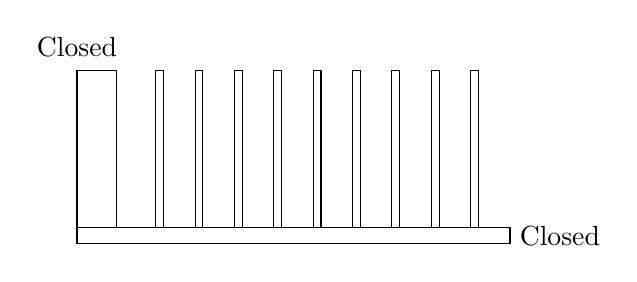
\begin{tikzpicture}
      \draw[black] (0,0)rectangle (0.5,2);
      \draw[black] (0,0)rectangle (5.5,-0.2);
      \foreach \x in {1,1.5,...,5}
      \draw[black] (\x,0)rectangle (\x+.1,2);
      \node [anchor=center] at (0,2.3) {Closed};
      \node [anchor=west] at (5.5,-.1) {Closed};
    \end{tikzpicture}
    \caption{Prediction 1 - Tank Closed, Valve Closed}
    \label{fig:prediction1}
  \end{center}
  \begin{center}
    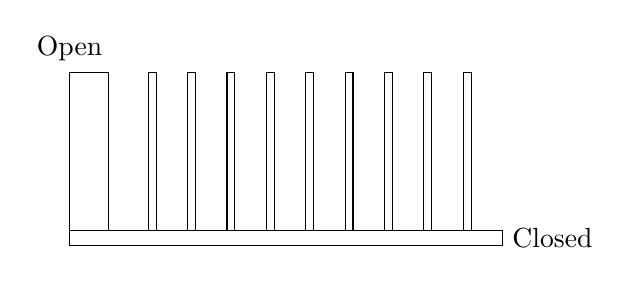
\begin{tikzpicture}
      \draw[black] (0,0)rectangle (0.5,2);
      \draw[black] (0,0)rectangle (5.5,-0.2);
      \foreach \x in {1,1.5,...,5}
      \draw[black] (\x,0)rectangle (\x+.1,2);
      \node [anchor=center] at (0,2.3) {Open};
      \node [anchor=west] at (5.5,-.1) {Closed};
    \end{tikzpicture}
    \caption{Prediction 2 - Tank Open, Valve Closed}
    \label{fig:prediction2}
  \end{center}
  \begin{center}
    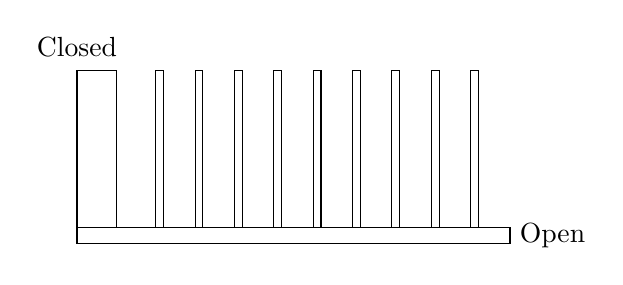
\begin{tikzpicture}
      \draw[black] (0,0)rectangle (0.5,2);
      \draw[black] (0,0)rectangle (5.5,-0.2);
      \foreach \x in {1,1.5,...,5}
      \draw[black] (\x,0)rectangle (\x+.1,2);
      \node [anchor=center] at (0,2.3) {Closed};
      \node [anchor=west] at (5.5,-.1) {Open};
    \end{tikzpicture}
    \caption{Prediction 3 - Tank Closed, Valve Open}
    \label{fig:prediction3}
  \end{center}
  \begin{center}
    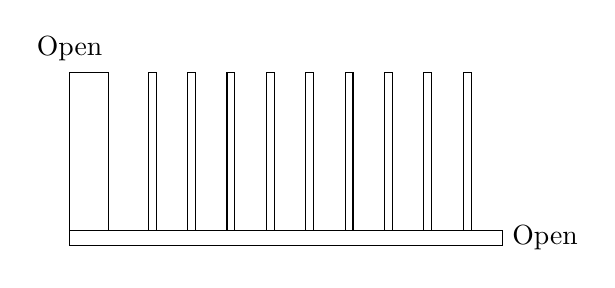
\begin{tikzpicture}
      \draw[black] (0,0)rectangle (0.5,2);
      \draw[black] (0,0)rectangle (5.5,-0.2);
      \foreach \x in {1,1.5,...,5}
      \draw[black] (\x,0)rectangle (\x+.1,2);
      \node [anchor=center] at (0,2.3) {Open};
      \node [anchor=west] at (5.5,-.1) {Open};
    \end{tikzpicture}
    \caption{Prediction 4 - Tank Open, Valve Open}
    \label{fig:prediction4}
  \end{center}
\end{figure}


\subsection{Equations}

\begin{align}
  v & = \sqrt{2gh} \label{eqn:efflux} \\
  gh & = \frac{1}{2}v^{2} \label{eqn:viva} \\
  gh & = v^{2} \label{eqn:vivas}
  % a^{2}+b^{2} & =c^{2}\\
% \textit{where } A & = 1 &&  \textit{A is measurement unit} \\
%   gh & = \frac{1}{2}Av^{2} \label{eqn:visflux} &&  \textit{Surface Area (A)} \\
%   [LT^{-2}][L] & = [L^2]^{0}[L^2T^{-2}] &&  \textit{Dimensions} \\
%   [L^2T^{-2}] & = 1 \times [L^2T^{-2}] \\
%   [L^5T^{-5}] & = [L^3T^{-3}] \times [L^2T^{-2}] &&  \textit{Power Dimensions} \\
%   [L^5T^{-5}] & = [L^3T^{-2}] \times [L^2T^{-2}] \times [T^{-1}]\\
%   [L^5T^{-5}] & = [M] \times [L^2T^{-2}] \times [T^{-1}]\\
%    P & = mv^{2} \times  \frac{1}{\tau}  \\
%     \textit{where, } \tau & = \frac{1}{k}  && \text{\cite[p.45]{odum_ecological_1994}} \\
%      P & = mv^{2} \times k \\
%      \textit{Living Power} & =  \textit{vis viva} \times \textit{Metabolic Constant} \\
%       \textit{however, } P & = p \times Av \\
     %  \textit{and, } \tau & = RC && \text{\cite[p.45]{odum_ecological_1994}} \\
     %  P & = \frac{mv^{2}}{RC}
\end{align}


\begin{figure}[h]
  \begin{center}
    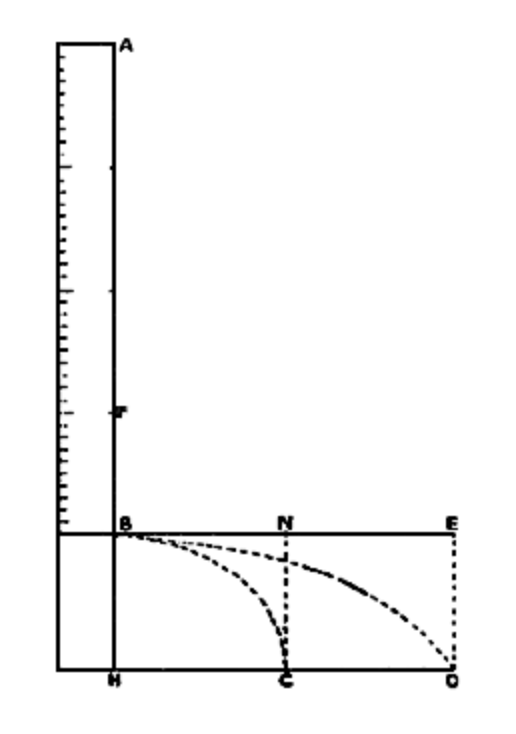
\includegraphics[width=0.35\textwidth]{DescartesWaterFlow} % Include the image placeholder.png
    \caption{Descartes force-flux}
    \label{fig:DescartesWaterFlow}
  \end{center}
\end{figure}

\begin{figure}[h]
\begin{center}
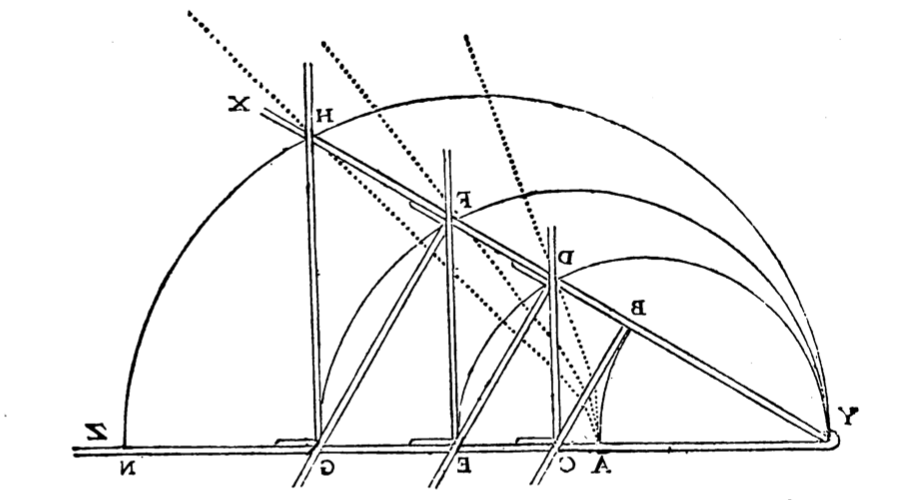
\includegraphics[width=0.75\textwidth]{idealInstrument} % Include the image placeholder.png
\caption{Descartes' ``Ideal machine''}
\label{fig:idealInstrument}
\end{center}
\end{figure}

\begin{figure}[h]
\begin{center}
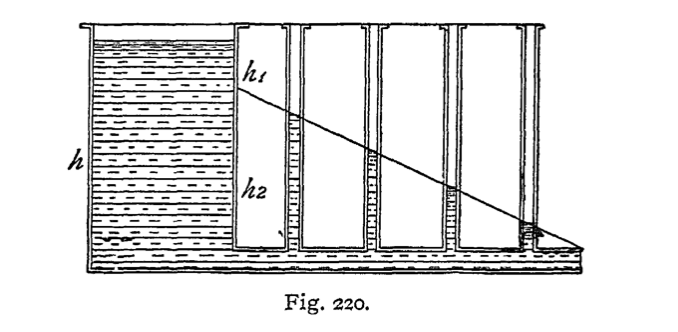
\includegraphics[width=0.75\textwidth]{machVenturi} % Include the image placeholder.png
\caption{Mach's Representation}
\label{fig:machVenturi}
\end{center}
\end{figure}


%----------------------------------------------------------------------------------------
%	SECTION 1
%----------------------------------------------------------------------------------------


% If you have more than one objective, uncomment the below:
%\begin{description}
%\item[First Objective] \hfill \\
%Objective 1 text
%\item[Second Objective] \hfill \\
%Objective 2 text
%\end{description}

\subsection{Definitions}
\label{definitions}
\begin{description}
  \item[Velocity]
  \dots
  \item[Gravity]
  \dots
  \item[Distance]
  \dots
\end{description}

%----------------------------------------------------------------------------------------
%	SECTION 2
%----------------------------------------------------------------------------------------

\section{Equipment}
\label{equipment}

\begin{tabular}{ll}
  Item & Quantity \\
  \hline \\
  Tank & 1 x 1L Water bottle \\
  Clear piping & 3 m x 4mm \\
  T-intersection & 1 Packet x 4mm (x 10 in pack) \\
  Tape & 1 x Roll Masking tape (or equiv.) \\
\end{tabular}

% \subsection{Apparatus}

\begin{figure}[h]
  \begin{center}
    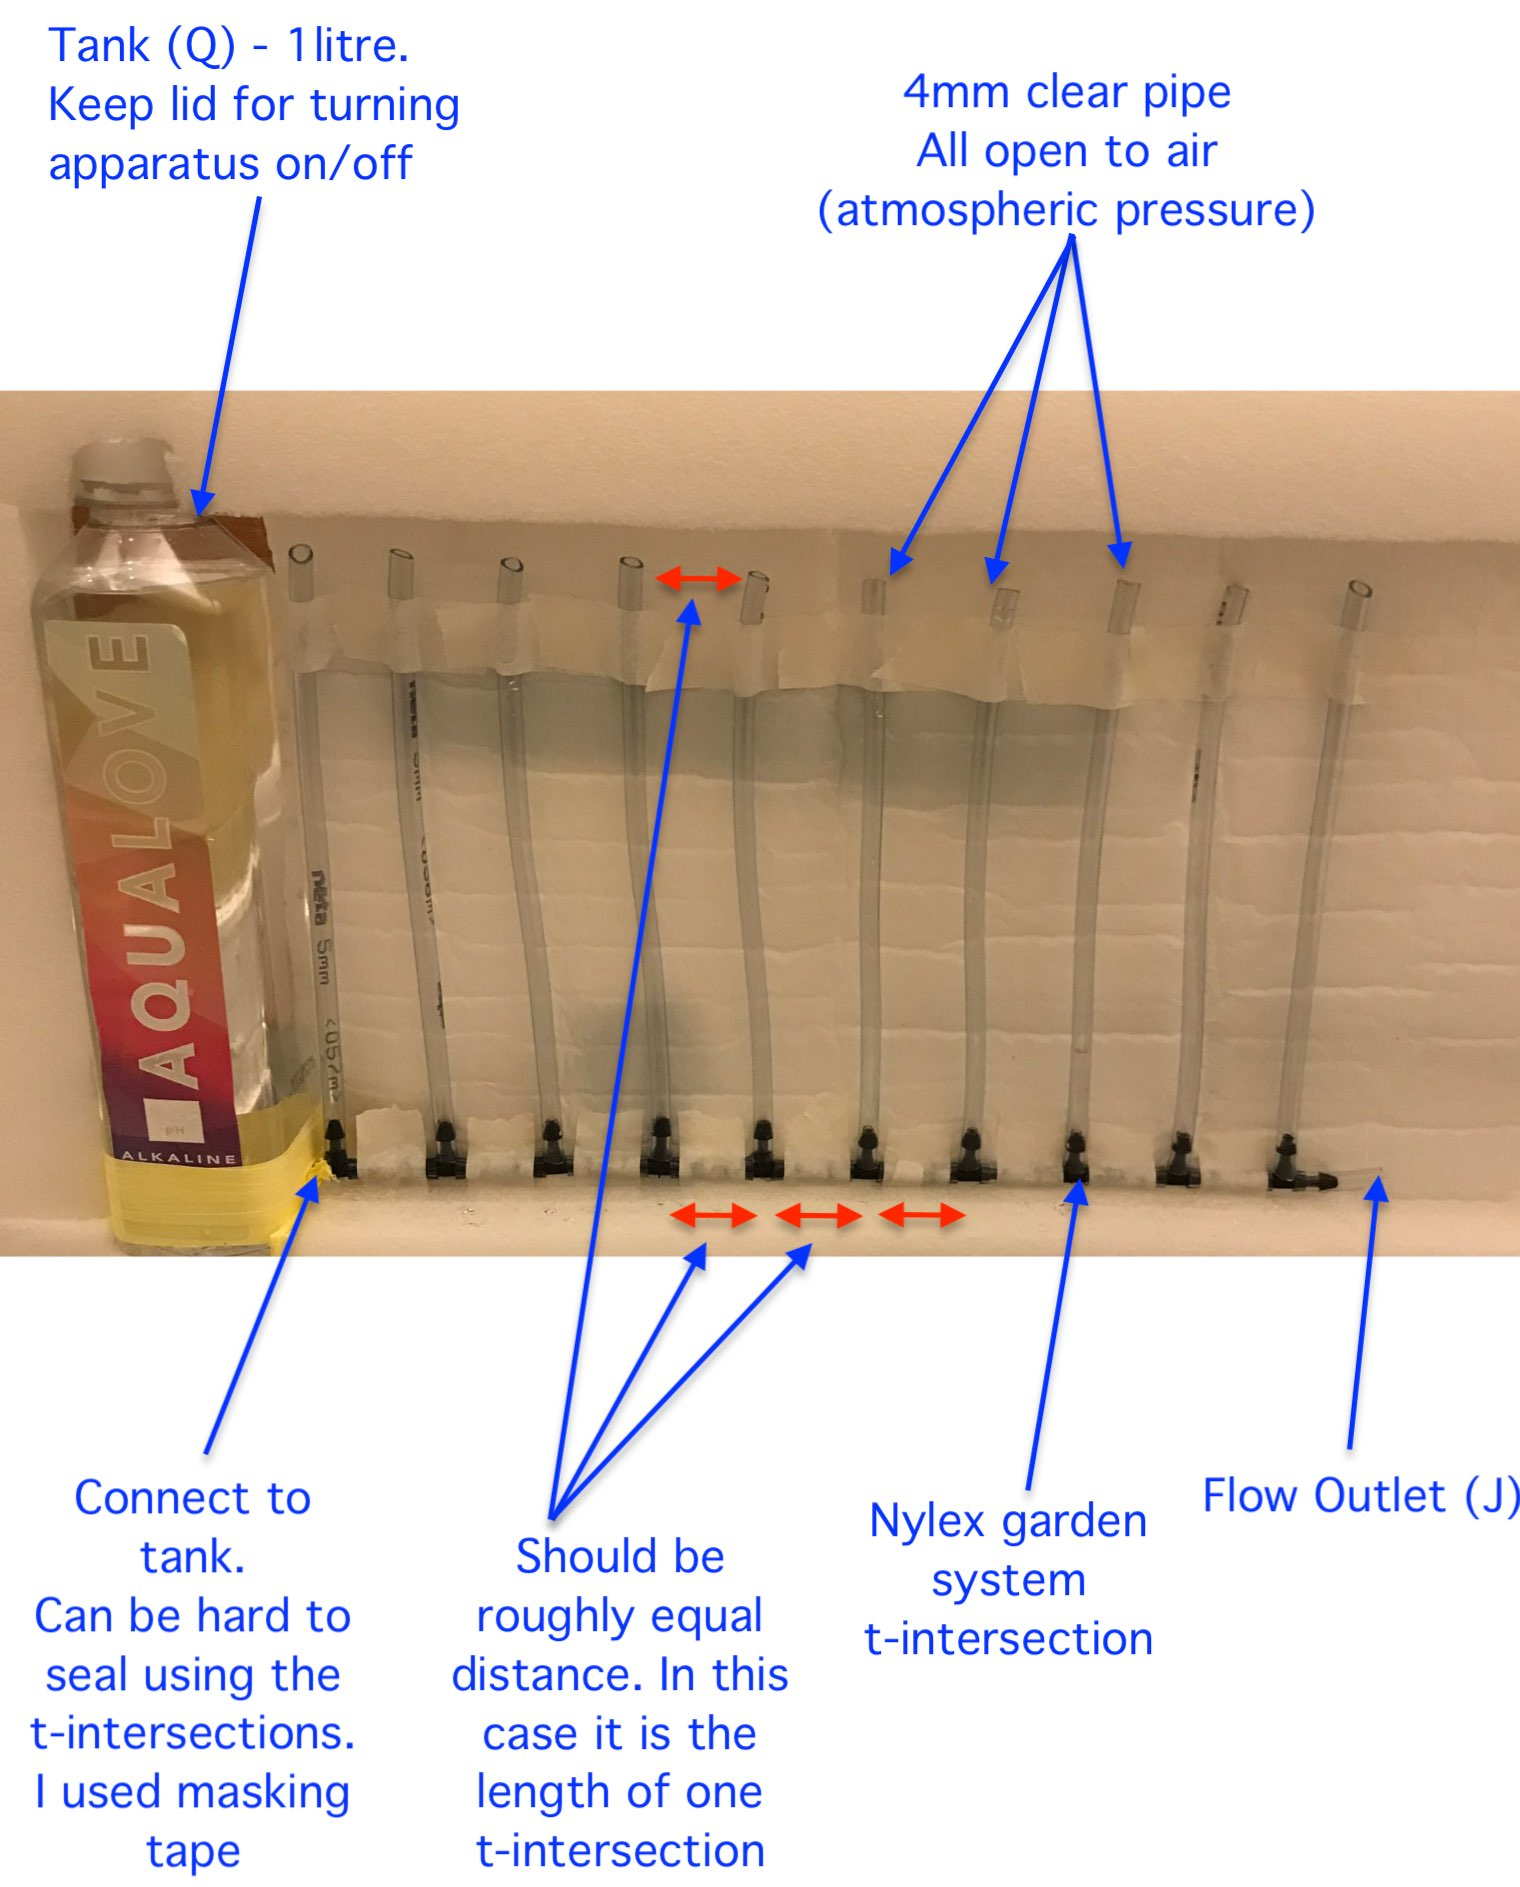
\includegraphics[width=0.75\textwidth]{full} % Include the image placeholder.png
    \caption{Full picture of apparatus}
    \label{fig:fullApparatus}
  \end{center}
\end{figure}

%
% \begin{figure}[h]
%   \begin{center}
%     % \includegraphics[width=0.75\textwidth]{Forces} % Include the image placeholder.png
%     \caption{Full picture of apparatus}
%     \label{fig:forcesApparatus}
%   \end{center}
% \end{figure}




%----------------------------------------------------------------------------------------
%	SECTION 2
%----------------------------------------------------------------------------------------

\section{Experimental Data}

\begin{tabular}{ll}
  Mass of 1 litre & $\rule{2cm}{0.15mm}$ (kilogram)\\
  Height of tank & $\rule{2cm}{0.15mm}$ (mm)\\
  Increments & $\rule{2cm}{0.15mm}$ (mm)\\
  Height of Vertical Measure Pipes & $\rule{2cm}{0.15mm}$  (mm)\\
  Total Length of Horizontal Pipe & $\rule{2cm}{0.15mm}$ (mm)\\
\end{tabular}

%----------------------------------------------------------------------------------------
%	SECTION 2
%----------------------------------------------------------------------------------------

\section{Method}

\subsection{Step 1}

Connect

\subsection{Step 2}

Take some baseline measurements of the amount of time the tank takes to empty when connected and not connected.

* Remember to catch the water for recycling.


\begin{tabular}{lll}
  Parameter & Apparatus State & Measurement \\
  \hline \\
  Time of emptying & tank disconnected & $\rule{2cm}{0.15mm}$ (sec)\\
  Time of emptying & tank connected & $\rule{2cm}{0.15mm}$ (sec)\\

\end{tabular}



%----------------------------------------------------------------------------------------
%	SECTION 3
%----------------------------------------------------------------------------------------

\section{Sample Calculation}

% \begin{tabular}{ll}
% Mass of magnesium metal & = \SI{8.59}{\gram} - \SI{7.28}{\gram}\\
% & = \SI{1.31}{\gram}\\
% Mass of magnesium oxide & = \SI{9.46}{\gram} - \SI{7.28}{\gram}\\
% & = \SI{2.18}{\gram}\\
% Mass of oxygen & = \SI{2.18}{\gram} - \SI{1.31}{\gram}\\
% & = \SI{0.87}{\gram}
% \end{tabular}

% Because of this reaction, the required ratio is the atomic weight of magnesium: \SI{16.00}{\gram} of oxygen as experimental mass of Mg: experimental mass of oxygen or $\frac{x}{1.31}=\frac{16}{0.87}$ from which, $M_{\ce{Mg}} = 16.00 \times \frac{1.31}{0.87} = 24.1 = \SI{24}{\gram\per\mole}$ (to two significant figures).

%----------------------------------------------------------------------------------------
%	SECTION 4
%----------------------------------------------------------------------------------------

\section{Results and Conclusions}
%
% The atomic weight of magnesium is concluded to be \SI{24}{\gram\per\mol}, as determined by the stoichiometry of its chemical combination with oxygen. This result is in agreement with the accepted value.
%
% \begin{figure}[h]
% \begin{center}
% 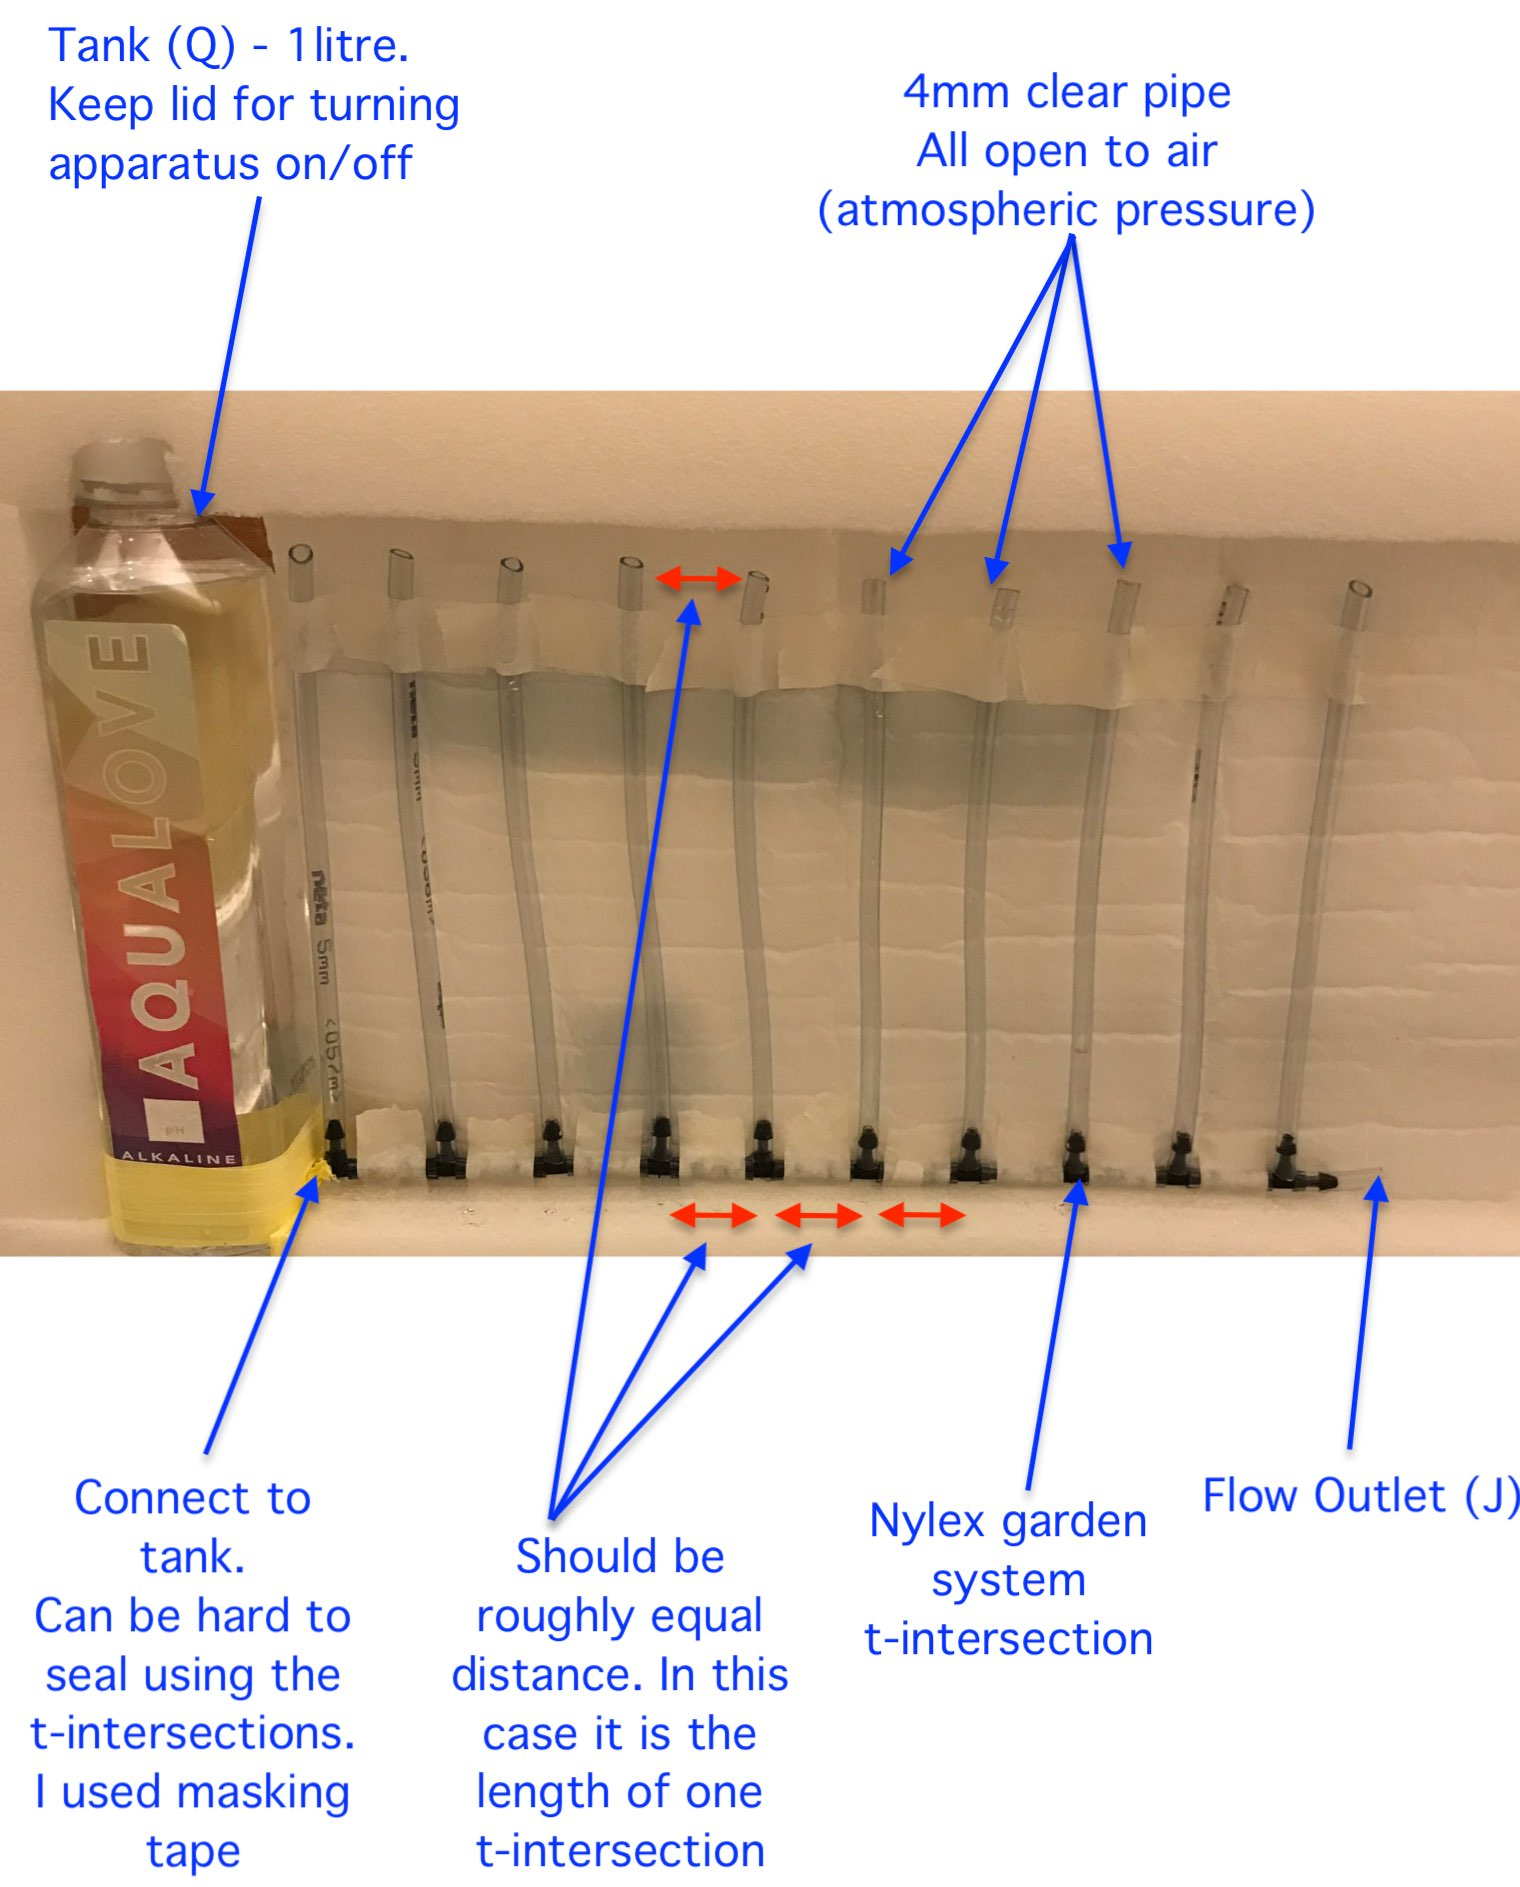
\includegraphics[width=0.35\textwidth]{full} % Include the image placeholder.png
% \caption{Full picture of apparatus}
% \label{fig:fullApparatus}
% \end{center}
% \end{figure}

%----------------------------------------------------------------------------------------
%	SECTION 5
%----------------------------------------------------------------------------------------

\section{Discussion of Experimental Uncertainty}

% The accepted value (periodic table) is \SI{24.3}{\gram\per\mole} \cite{Smith:2012qr}. The percentage discrepancy between the accepted value and the result obtained here is 1.3\%. Because only a single measurement was made, it is not possible to calculate an estimated standard deviation.
%
% The most obvious source of experimental uncertainty is the limited precision of the balance. Other potential sources of experimental uncertainty are: the reaction might not be complete; if not enough time was allowed for total oxidation, less than complete oxidation of the magnesium might have, in part, reacted with nitrogen in the air (incorrect reaction); the magnesium oxide might have absorbed water from the air, and thus weigh ``too much." Because the result obtained is close to the accepted value it is possible that some of these experimental uncertainties have fortuitously cancelled one another.

%----------------------------------------------------------------------------------------
%	SECTION 6
%----------------------------------------------------------------------------------------

\section{Answers to Definitions}
%
% \begin{enumerate}
% \begin{item}
% The \emph{atomic weight of an element} is the relative weight of one of its atoms compared to C-12 with a weight of 12.0000000$\ldots$, hydrogen with a weight of 1.008, to oxygen with a weight of 16.00. Atomic weight is also the average weight of all the atoms of that element as they occur in nature.
% \end{item}
% \begin{item}
% The \emph{units of atomic weight} are two-fold, with an identical numerical value. They are g/mole of atoms (or just g/mol) or amu/atom.
% \end{item}
% \begin{item}
% \emph{Percentage discrepancy} between an accepted (literature) value and an experimental value is
% \begin{equation*}
% \frac{\mathrm{experimental\;result} - \mathrm{accepted\;result}}{\mathrm{accepted\;result}}
% \end{equation*}
% \end{item}
% \end{enumerate}

%----------------------------------------------------------------------------------------
%	BIBLIOGRAPHY
%----------------------------------------------------------------------------------------

\bibliographystyle{apalike}

\bibliography{references}

%----------------------------------------------------------------------------------------


\end{document}
